\documentclass[convert={density=300,outext=.png}]{standalone}
\usepackage{tikz}
\usetikzlibrary{patterns,decorations.pathmorphing,positioning}
\begin{document}
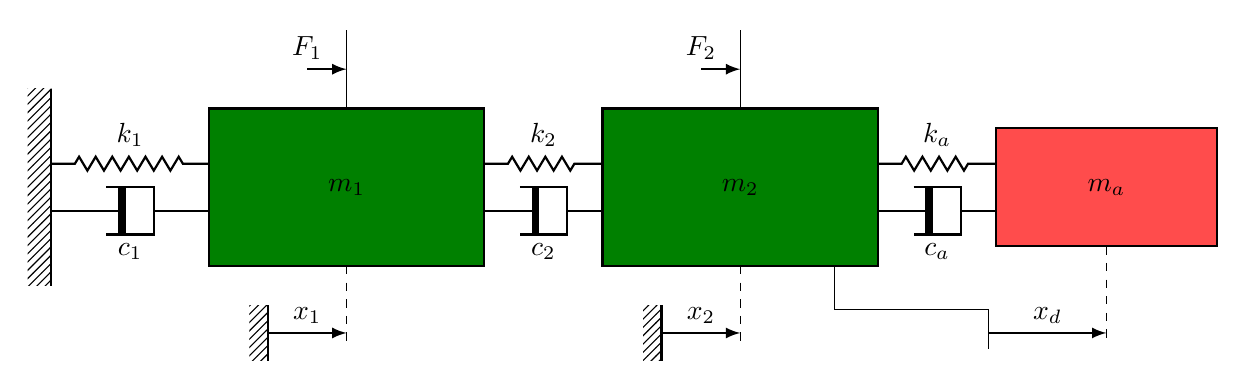
\begin{tikzpicture}[every node/.style={outer sep=0pt},thick,
 mass/.style={draw,thick},
 spring/.style={thick,decorate,decoration={zigzag,pre length=0.3cm,post
 length=0.3cm,segment length=6}},
 ground/.style={fill,pattern=north east lines,draw=none,minimum
 width=0.75cm,minimum height=0.3cm},
 dampic/.pic={\fill[white] (-0.1,-0.3) rectangle (0.3,0.3);
 \draw (-0.3,0.3) -| (0.3,-0.3) -- (-0.3,-0.3);
 \draw[line width=1mm] (-0.1,-0.3) -- (-0.1,0.3);}]

  \node[mass,minimum width=3.5cm,minimum height=2cm,fill=green!50!black] (m1) {$m_1$};
  \node[mass,minimum width=3.5cm,minimum height=2cm,fill=green!50!black,right=1.5cm of
  m1] (m2) {$m_2$};
  \node[mass,minimum width=2.8cm,minimum height=1.5cm,fill=red!70,right=1.5cm of
  m2] (ma) {$m_a$};
  \node[left=2cm of m1,ground,minimum width=3mm,minimum height=2.5cm] (g1){};
  \draw (g1.north east) -- (g1.south east);

  \draw[spring] ([yshift=3mm]g1.east) coordinate(aux)
   -- (m1.west|-aux) node[midway,above=1mm]{$k_1$};
  \draw[spring]  (m1.east|-aux) -- (m2.west|-aux) node[midway,above=1mm]{$k_2$};
  \draw[spring]  (m2.east|-aux) -- (ma.west|-aux) node[midway,above=1mm]{$k_a$};

  \draw ([yshift=-3mm]g1.east) coordinate(aux')
   -- (m1.west|-aux') pic[midway]{dampic} node[midway,below=3mm]{$c_1$}
     (m1.east|-aux') -- (m2.west|-aux') pic[midway]{dampic} node[midway,below=3mm]{$c_2$}
     (m2.east|-aux') -- (ma.west|-aux') pic[midway]{dampic} node[midway,below=3mm]{$c_a$};

  \foreach \X in {1,2}  
  {\draw[thin] (m\X.north) -- ++ (0,1) coordinate[midway](aux\X);
   \draw[latex-] (aux\X) -- ++ (-0.5,0) node[above]{$F_\X$}; 
   \draw[thin,dashed] (m\X.south) -- ++ (0,-1) coordinate[pos=0.85](aux'\X);
   \draw[latex-] (aux'\X) -- ++ (-1,0) node[midway,above]{$x_\X$}
    node[left,ground,minimum height=7mm,minimum width=1mm] (g'\X){};
   \draw[thick] (g'\X.north east) -- (g'\X.south east);
  }

  \draw[thin,dashed] (ma.south) -- ++(0,-1.2);
  \draw[latex-] (ma.south |- aux'1) -- ++ (-1.5,0) coordinate(aux3)
  node[midway,above]{$x_d$};
  \draw[thin] ([yshift=-2mm]aux3) |- ++ (-1,0.5) -| (m2.-40);
\end{tikzpicture}
\end{document}
